% !TeX root = probability.tex

%%%%%%%%%%%%%%%%%%%%%%%%%%%%%%%%%%%%%%%%%%%%%%%%%%%%%%%%%%%%%

\section{קיץ תשע"ו מועד ב}

\begin{center}
\selectlanguage{english}
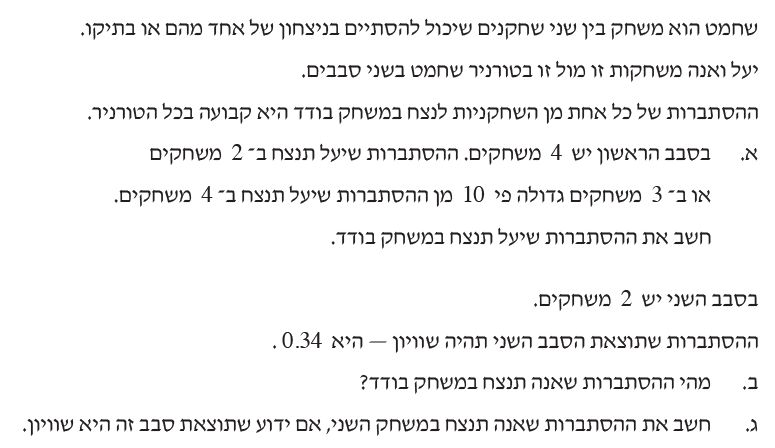
\includegraphics[width=.86\textwidth]{summer-2016b-3}
\end{center}

\textbf{סעיף א}

נסמן את המאורע "יעל תנצח במשחק בודד" ב-%
$Y$ \L{(Yael)}
ונסמן
$y=P(Y)$.
הצלחה מוגדרת על ידי ניצחונות של יעל והשאלה מספקת מידע על מספרי ההצלחות ולכן נשמתמש בנוסחת ברנולי:
\begin{eqn}
{4 \choose 2}y^2(1-y)^2 + {4\choose 3}y^3(1-y) &=& 10\cdot {4\choose 4}y^4(1-y)^0\\
8y^2+8y-6&=&0\\
y&=&\frac{1}{2}\,,
\end{eqn}
ונתעלם מהשורש השני 
$-\frac{3}{2}$
כי הסתברות לא יכולה להיות שלילי.

\textbf{סעיף ב}

נסמן את המאורע "אנה תנצח במשחק בודד" ב-%
$A$ \L{(Anna)}
ונסמן
$a=P(A)$.

נסמן ב-%
$S$ \L{(shivyon)}
את המאורע שתוצאת הסבב השני תהיה תיקו. האפשרויות לקבל שוויון הן ניצחון אחד לאנה וליעל בהסתברות 
$ya+ay$,
או תיקו בשני המשחקים בהסתברות
$(1-(y+a))^2$
כי ההסתברות לתיקו במשחק אחד היא המשלים לסכום ההסתברויות שאחת מהן תנצח. נציב
$y=\frac{1}{2}$
והמידע ש-%
$P(S)=0.34$
ונקבל:
\begin{eqn}
{2 \choose 1}ya + (1-(y+a))^2 &=&P(S)= 0.34\\
a + (\textstyle\frac{1}{2}-a)^2&=&0.34\\
a&=&0.3\,,
\end{eqn}
כאשר נתעלם מהשורש
$-0.3$
כי הסתברות לא יכולה להיות שלילית.

\textbf{סעיף ג}

נסמן את המאורע "אנה תנצח במשחק השני" ב-%
$A2$.

הניסוח
"\textbf{אם ידוע ש-}"
מכוון להסתברות מותנית:
\begin{eqn}
P(A2/S) &=& \frac{P(A2\:\cap\;S)}{P(S)}\\
&=&\frac{ya}{P(S)}=\frac{0.5\cdot 0.3}{0.34}=0.4412\,.
\end{eqn}

ההסתברות לשיוון בסבב השני נתונה. אם אנה תנצח במשחק השני, יהיה שוויון רק אם גם יעל תנצח במשחק הראשון:
\[
\frac{ya}{.34}=\frac{0.5\cdot 0.3}{.34}=0.4412\,.
\]
שימו לב שאם יש שיוון ואנה מנצחת במשחק הראשון, יעל חייבת לנצח במשחק הראשון ולכם המנה היא 
$ya$.

%%%%%%%%%%%%%%%%%%%%%%%%%%%%%%%%%%%%%%%%%%%%%%%%%%%%%%%%%%%%%%

\newpage

\section{קיץ תשע"ו מועד א}

\begin{center}
\selectlanguage{english}
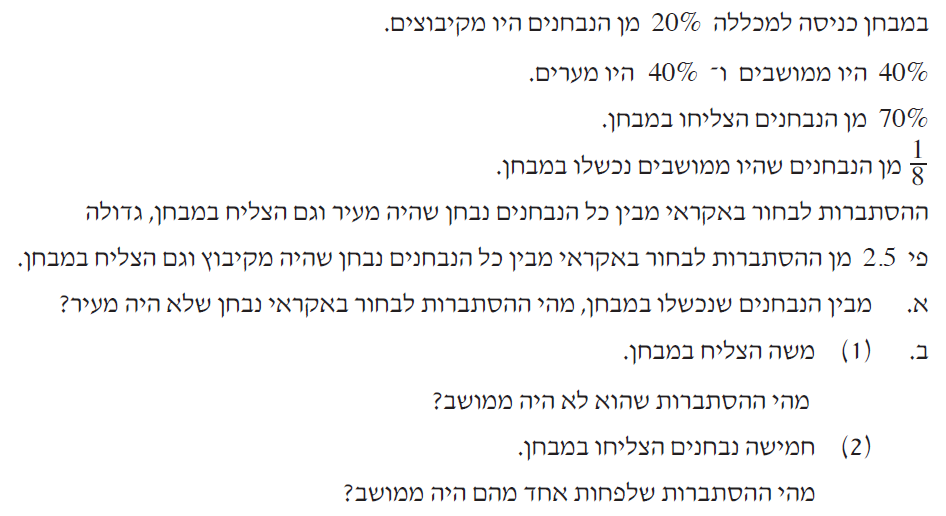
\includegraphics[width=.95\textwidth]{summer-2016a-3}
\end{center}

נסמן את המאורעות השונים בשאלה.
\begin{itemize}
\item $S$ \L{(success)}
הנבחנים שהצליחו.
\item $K$ \L{(kibbutz)} 
נבחנים מקיבוצים.
\item $M$ \L{(moshav)}
נבחנים ממושבים.
\item $E$ \L{(eer)}
נבחנים מערים.
\end{itemize}
ההסתברויות של המאורעות הללו נתונות:
\[
P(K)=0.20,\;P(M)=0.40,\;P(E)=0.40,\;P(S)=0.70\,.
\]
בשאלה שני סוגים של קבוצות: הצלחת הנבחנים ומקום המגורים של הנבחנים ולכן נשתמש בטבלה:
\begin{center}
\selectlanguage{english}
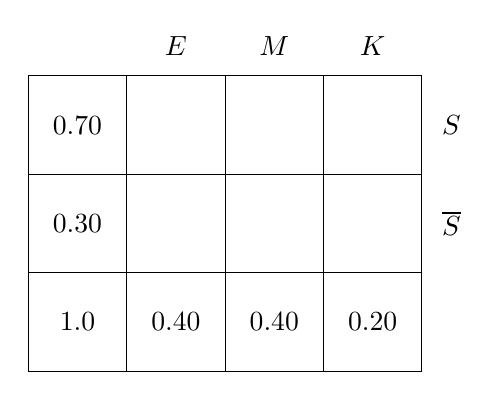
\begin{tikzpicture}[scale=1.25]
\draw (0,0) grid (4,3);
\node at (3.5,3.3) {$K$};
\node at (2.5,3.3) {$M$};
\node at (1.5,3.3) {$E$};
\node at (4.3,2.5) {$S$};
\node at (4.3,1.5) {$\overline{S}$};

\node at (0.5,2.5) {$0.70$};
\node at (0.5,1.5) {$0.30$};
\node at (0.5,0.5) {$1.0$};

%\node at (1.5,2.5) {$0.25$};
%\node at (1.5,1.5) {$0.15$};
\node at (1.5,0.5) {$0.40$};

%\node at (2.5,2.5) {$0.35$};
%\node at (2.5,1.5) {$0.05$};
\node at (2.5,0.5) {$0.40$};

%\node at (3.5,2.5) {$0.10$};
%\node at (3.5,1.5) {$0.10$};
\node at (3.5,0.5) {$0.20$};
\end{tikzpicture}
\end{center}
מידע נוסף שניתן הוא "%
$\frac{1}{8}$
\textbf{מן הנבחנים}
שהיו ממושבים נכשלו במבחן", כאשר הניסוח מכוון להסתברות מותנית. נחשב:
\begin{eqn}
P(\overline{S}/M)&=&P(\overline{S}\cap M) / P(M)\\
P(\overline{S}\cap M)&=&P(\overline{S}/M)\cdot P(M)=\frac{1}{8}\cdot 0.40=0.05\,.
\end{eqn}
הנתון האחרון מתקבל מהפסקאות "ההסתברות לבחור באקראי
\textbf{מבין כל}
הנבחנים נבחן שהיה ב-%
$\cdots$
\textbf{וגם}
הצליח במבחן". הניסוח מכוון לחיתוך הסתברויות, ולכן הנתון הוא
$P(E\cap S)=2.5\cdot P(K\cap S)$.

נחשב את 
$P(S)=0.70$
על ידי סיכום ההסתברויות של המצליחים במבחן בכל מקום מגורים:
\begin{eqn}
P(S)&=&P(K\cap S)+P(M \cap S) + P(K\cap E)\\
0.70&=&P(K\cap S)+ 0.35 + 2.5\cdot P(K\cap S)\\
P(K\cap S)&=&0.10\\
P(E\cap S)&=&0.25\,.
\end{eqn}
נשלים את הטבלה:
\begin{center}
\selectlanguage{english}
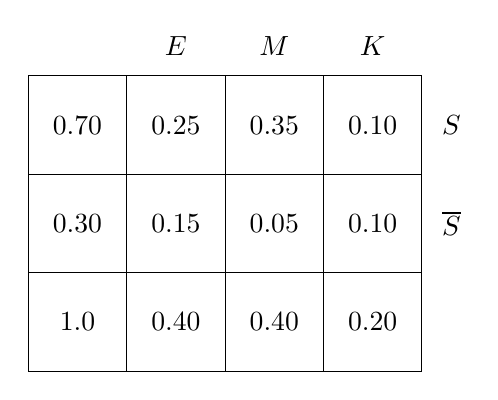
\begin{tikzpicture}[scale=1.25]
\draw (0,0) grid (4,3);
\node at (3.5,3.3) {$K$};
\node at (2.5,3.3) {$M$};
\node at (1.5,3.3) {$E$};
\node at (4.3,2.5) {$S$};
\node at (4.3,1.5) {$\overline{S}$};

\node at (0.5,2.5) {$0.70$};
\node at (0.5,1.5) {$0.30$};
\node at (0.5,0.5) {$1.0$};

\node at (1.5,2.5) {$0.25$};
\node at (1.5,1.5) {$0.15$};
\node at (1.5,0.5) {$0.40$};

\node at (2.5,2.5) {$0.35$};
\node at (2.5,1.5) {$0.05$};
\node at (2.5,0.5) {$0.40$};

\node at (3.5,2.5) {$0.10$};
\node at (3.5,1.5) {$0.10$};
\node at (3.5,0.5) {$0.20$};
\end{tikzpicture}
\end{center}
\textbf{סעיף א}

לפי הנוסחה להסתברות מותנית:
\[
P(\overline{E}/\overline{S})=P((K\cup M)/\overline{S}) = \frac{P(K\cap \overline{S})+P(M\cap \overline{S})}{P(\overline{S})}=\frac{0.10+0.05}{0.30}=\frac{1}{2}\,.
\]
\textbf{(1) סעיף ב}

לפי הנוסחה להסתברות מותנית:
\[
P(\overline{M}/S)=P((K\cup E)/S) = \frac{P(K\cap S)+P(E\cap S)}{P(S)}=\frac{0.10+0.25}{0.70}=\frac{1}{2}\,.
\]
\textbf{(2) סעיף ב}

"לפחות אחד ממושב" הוא המשלים ל-"כולם לא מהמושב" ולפי נוסחת ברנולי:
\[
1-P(\overline{M}/S)^5=1-\left(\frac{1}{2}\right)^2=\frac{31}{32}\,.
\]

%%%%%%%%%%%%%%%%%%%%%%%%%%%%%%%%%%%%%%%%%%%%%%%%%%%%%%%%%%%%

\section{חורף תשע"ו}

\begin{center}
\selectlanguage{english}
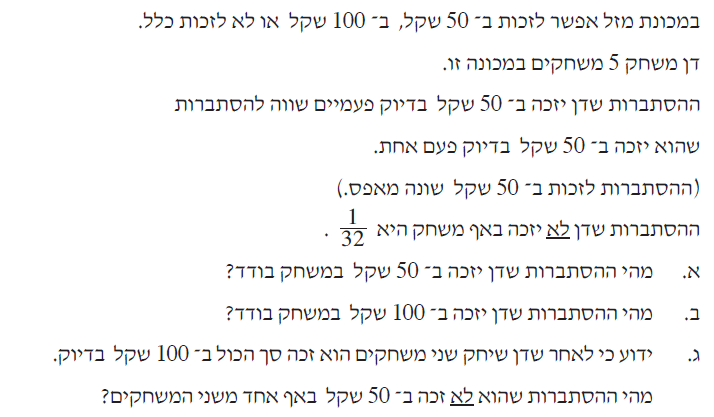
\includegraphics[width=.85\textwidth]{winter-2016-3}
\end{center}

המאורעות הם סכומי הכסף שדן זכה 
$0,50,100$.
נסמן ב-%
$P(n)$
את ההסתברות שדן זכה ב-%
$n$.

\textbf{סעיף א}

הניסוחים "אף אחד" ו-"בדיוק" מכוונים לנוסחת ברנולי. ההסתברות שדן לא זכה (בסכום חיובי) באף אחד מחמישת המשחקים היא 
$P(0)^5=\frac{1}{32}$
ולכן 
$P(0)=\frac{1}{2}$.
לפי המידע הנתון:
\begin{eqn}
{5\choose 2} P(50)^2 (1-P(50))^3 &=& {5\choose 1} P(50) (1-P(50))^4\\
10P(50)&=&5(1-P(50))\\
P(50)&=&\frac{1}{3}\,.
\end{eqn}

\textbf{סעיף ב}

לפי ההסתברות המשלימה:
$P(100) = 1 - P(0) - P(50) = 1-\frac{1}{2}-\frac{1}{3}=\frac{1}{6}$.



\textbf{סעיף ג}

נסמן ב-%
$M2$
את המאורע שדן זכה ב-%
$100$
בשני משחקים ונסמן ב-%
$\overline{50}$
את המאורע שדן לא זכה ב-%
$50$.
הניסוח
"\textbf{ידוע כי}"
מכוון להסתברות מותנית:
\[
P(\overline{50}/M2)=\frac{P(\overline{50}\cap M2)}{P(M2)}
\]
המשחקים מתרחשים אחד אחרי השני ולא לתלויים אחד בשני ולכן ניתן להציג את ההסתברויות בעץ (בעמוד הבא). בסוף כל מסלול רשום המאורעות 
$M2,\overline{50}$
שמתקיימים. ההסתברות המותנית היא:
\[
\frac{\frac{1}{2}\cdot\frac{1}{6} + \frac{1}{6}\cdot \frac{1}{2}}{\frac{1}{2}\cdot\frac{1}{6} + \frac{1}{3}\cdot \frac{1}{3}+ \frac{1}{6}\cdot \frac{1}{2}}  =  \frac{\frac{1}{6}}{\frac{5}{18}}=\frac{3}{5}\,.
\]

\begin{center}
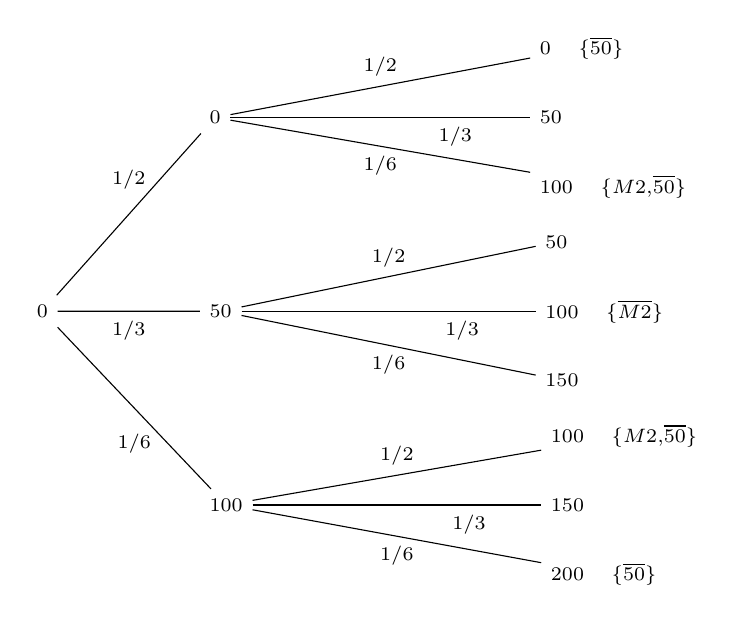
\begin{tikzpicture}
[grow=right,
level 1/.append style={level distance=2cm,
                       sibling distance=7em},
level 2/.append style={level distance=4cm,
                       sibling distance=2.5em}]
\node[left] {$\scriptstyle 0$} % root
child {
  node[right] {$\scriptstyle 100$}
    child {
      node[right] {$\scriptstyle 200\quad \{\overline{50}\}$}
      edge from parent node[below] {$\scriptstyle 1/6$}
    }
    child {
      node[right] {$\scriptstyle 150$}
      edge from parent node[below,near end] {$\scriptstyle 1/3$}
    }
    child {
      node[right] {$\scriptstyle 100\quad \{M2,\overline{50}\}$}
      edge from parent node[above] {$\scriptstyle 1/2$}
    }
    edge from parent node[below,yshift=-2mm] {$\scriptstyle 1/6$}
}
child {
  node[right] {$\scriptstyle 50$}
    child {
      node[right] {$\scriptstyle 150$}
      edge from parent node[below] {$\scriptstyle 1/6$}
    }
    child {
      node[right] {$\scriptstyle 100\quad \{\overline{M2}\}$}
      edge from parent node[below,near end] {$\scriptstyle 1/3$}
    }
    child {
      node[right] {$\scriptstyle 50$}
      edge from parent node[above] {$\scriptstyle 1/2$}
    }
    edge from parent node[below] {$\scriptstyle 1/3$}
}
child {
  node[right] {$\scriptstyle 0$}
    child {
      node[right] {$\scriptstyle 100\quad \{M2,\overline{50}\}$}
      edge from parent node[below] {$\scriptstyle 1/6$}
    }
    child {
      node[right] {$\scriptstyle 50$}
      edge from parent node[below,near end] {$\scriptstyle 1/3$}
    }
    child {
      node[right] {$\scriptstyle 0\quad \{\overline{50}\}$}
      edge from parent node[above] {$\scriptstyle 1/2$}
    }
    edge from parent node[above,yshift=2mm] {$\scriptstyle 1/2$}
}
;
\end{tikzpicture}
\end{center}

